%レイアウトの都合上newpageしない
\section{LEDの明るさを変える}
HSPスクリプトエディタで\textasciitilde /05/pwm.hspを開いて実行してください。\\

\begin{lstlisting}[caption=pwm.hsp,label=pwm.hsp]
#include "hsp3dish.as"
#include "rpz-gpio.as"

redraw 0
redraw 1

repeat
gpio 27,1

<#red#repeat 200
if cnt < 10 : gpio 17,1 : else : gpio 17,0
if cnt < 50 : gpio 18,1 : else : gpio 18,0
if cnt < 100 : gpio 22,1 : else : gpio 22,0
loop#>

await 1
loop

gpio 17,0
gpio 18,0
gpio 22,0
gpio 27,0
stop

\end{lstlisting}

緑色のLEDは明るさが弱く、白色のLEDは明るさが強くなっています。LEDを光らせるためには1、消すためには0を使います。1秒や2秒ごとに1と0を切りかえると、LEDが点いたり消えたりするのが人間でもわかります。プログラムがもっと高速に1と0を切りかえると、人間には\ruby{点滅}{てん|めつ}がわからなくなり、LEDがずっと光っているように見えます。このことを利用して、LEDの点灯時間の\ruby{比率}{ひ|りつ}を変えて明るさに強弱をつけることができます。

\begin{figure}[H]
\centering
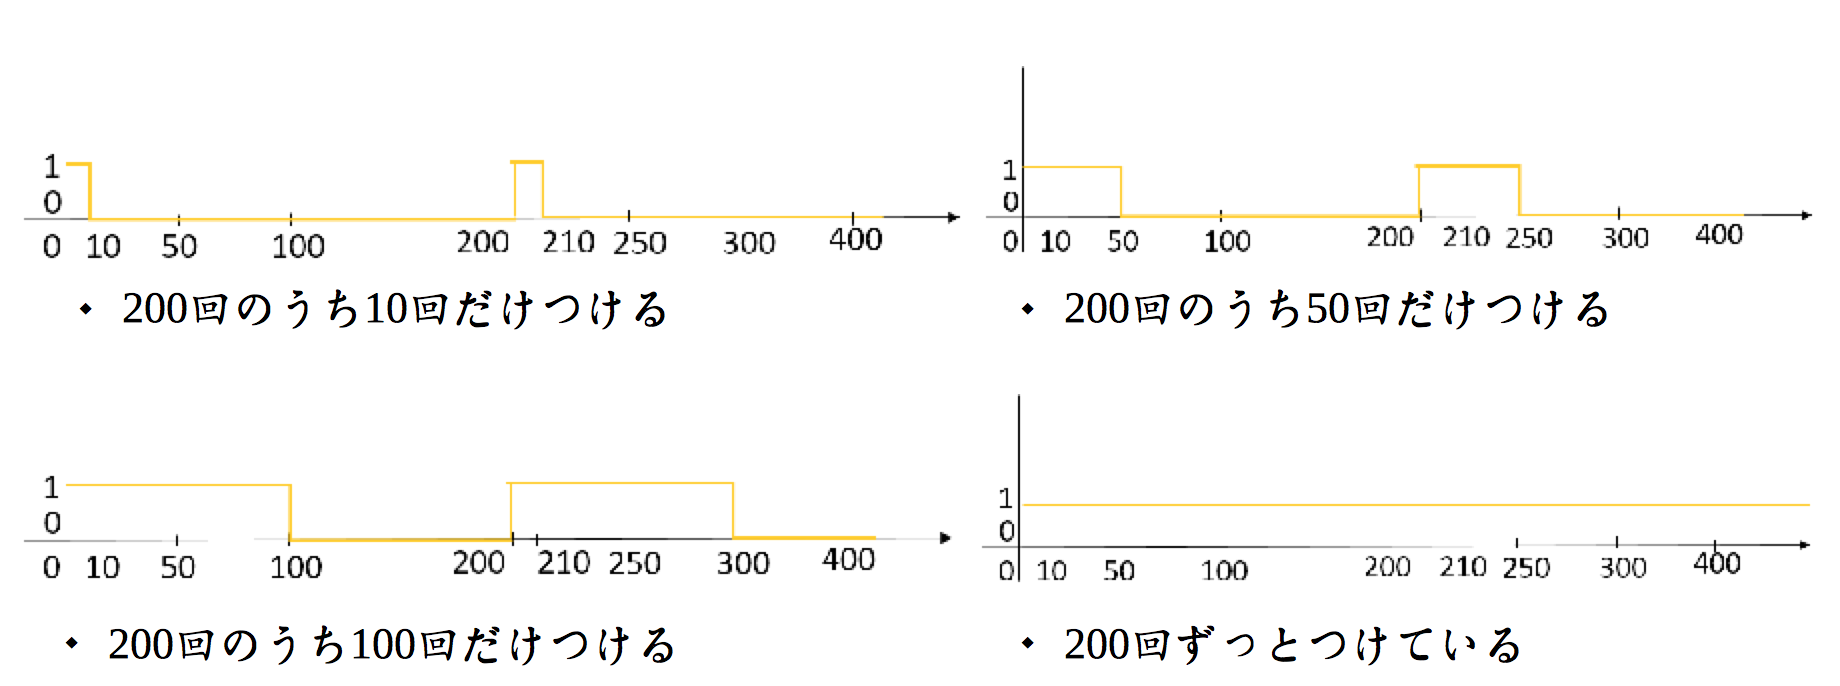
\includegraphics[scale=0.5]{images/chap05/text05-img035.png}
\caption{PWM}
\end{figure}

10行目から14行目の文字が赤くなっている部分を見てみましょう。repeat 200で3つのif文を200回\ruby{繰}{く}り返しています。GPIO17はカウントが10より小さいときだけLEDをつけます。200回のうち10回しかつけていないので、光が弱くなっています。GPIO22はカウントが100回より小さいときLEDをつけます。200回のうち100回もLEDをつけているので、GPIO22につながっているLEDはGPIO17につながっているLEDより強く光ります。